% Chapter 2. What the handshake bought, and what deleting it bought.
\documentclass[tikz,border=6pt]{standalone}
% Shared look for every TikZ figure in the book.
% Colours match book/preamble.tex exactly. Change both or neither.

\usepackage{tikz}
\usepackage{xcolor}
\usepackage{amsmath}
\IfFileExists{libertinus.sty}{\usepackage[mono=false]{libertinus}}{}
\IfFileExists{inconsolata.sty}{\usepackage[varqu,varl,scaled=0.95]{inconsolata}}{}

\usetikzlibrary{
  arrows.meta, positioning, calc, fit, backgrounds, shapes.geometric,
  shapes.misc, decorations.pathreplacing, decorations.pathmorphing,
  patterns, chains, matrix, shadows.blur
}

\definecolor{ink}{HTML}{15181D}
\definecolor{muted}{HTML}{5B6472}
\definecolor{rule}{HTML}{C9CED6}
\definecolor{wash}{HTML}{F4F5F7}
\definecolor{accent}{HTML}{0F5C8C}
\definecolor{accentsoft}{HTML}{E7F0F6}
\definecolor{warm}{HTML}{B4531A}
\definecolor{warmsoft}{HTML}{FBF0E7}
\definecolor{good}{HTML}{2C6E49}
\definecolor{goodsoft}{HTML}{E9F2EC}
\definecolor{danger}{HTML}{9B2226}
\definecolor{dangersoft}{HTML}{FAECEC}

\tikzset{
  font=\sffamily\small,
  >={Stealth[length=5pt, width=4pt]},
  %
  box/.style={
    draw=rule, line width=0.8pt, fill=wash, rounded corners=2pt,
    inner sep=7pt, align=center, text=ink, minimum height=9mm,
  },
  boxa/.style={box, draw=accent, fill=accentsoft},
  boxg/.style={box, draw=good,   fill=goodsoft},
  boxw/.style={box, draw=warm,   fill=warmsoft},
  boxd/.style={box, draw=danger, fill=dangersoft},
  %
  lane/.style={draw=rule, line width=0.7pt, fill=white, rounded corners=2pt,
               inner sep=6pt, align=center, minimum width=26mm},
  %
  flow/.style={draw=accent, line width=1.0pt, ->},
  flowback/.style={flow, densely dashed},
  flowmuted/.style={draw=muted, line width=0.8pt, ->},
  lifeline/.style={draw=rule, line width=0.7pt, densely dotted},
  %
  lbl/.style={font=\sffamily\scriptsize, text=muted, inner sep=2pt},
  lblink/.style={font=\sffamily\scriptsize, text=ink, inner sep=2pt},
  tag/.style={font=\ttfamily\scriptsize, text=accent, inner sep=2pt,
              fill=white, inner xsep=3pt},
  note/.style={font=\sffamily\scriptsize\itshape, text=muted, align=left},
  %
  band/.style={draw=none, rounded corners=1pt},
  tick/.style={draw=muted, line width=0.6pt},
}

% A horizontal timeline bar segment: \barseg{x0}{x1}{y}{colour}{label}
\newcommand{\barseg}[5]{%
  \fill[#4, rounded corners=1pt] (#1,#3-0.16) rectangle (#2,#3+0.16);
  \node[lbl, text=white, font=\sffamily\scriptsize\bfseries]
       at ({(#1+#2)/2},#3) {#5};
}

\begin{document}
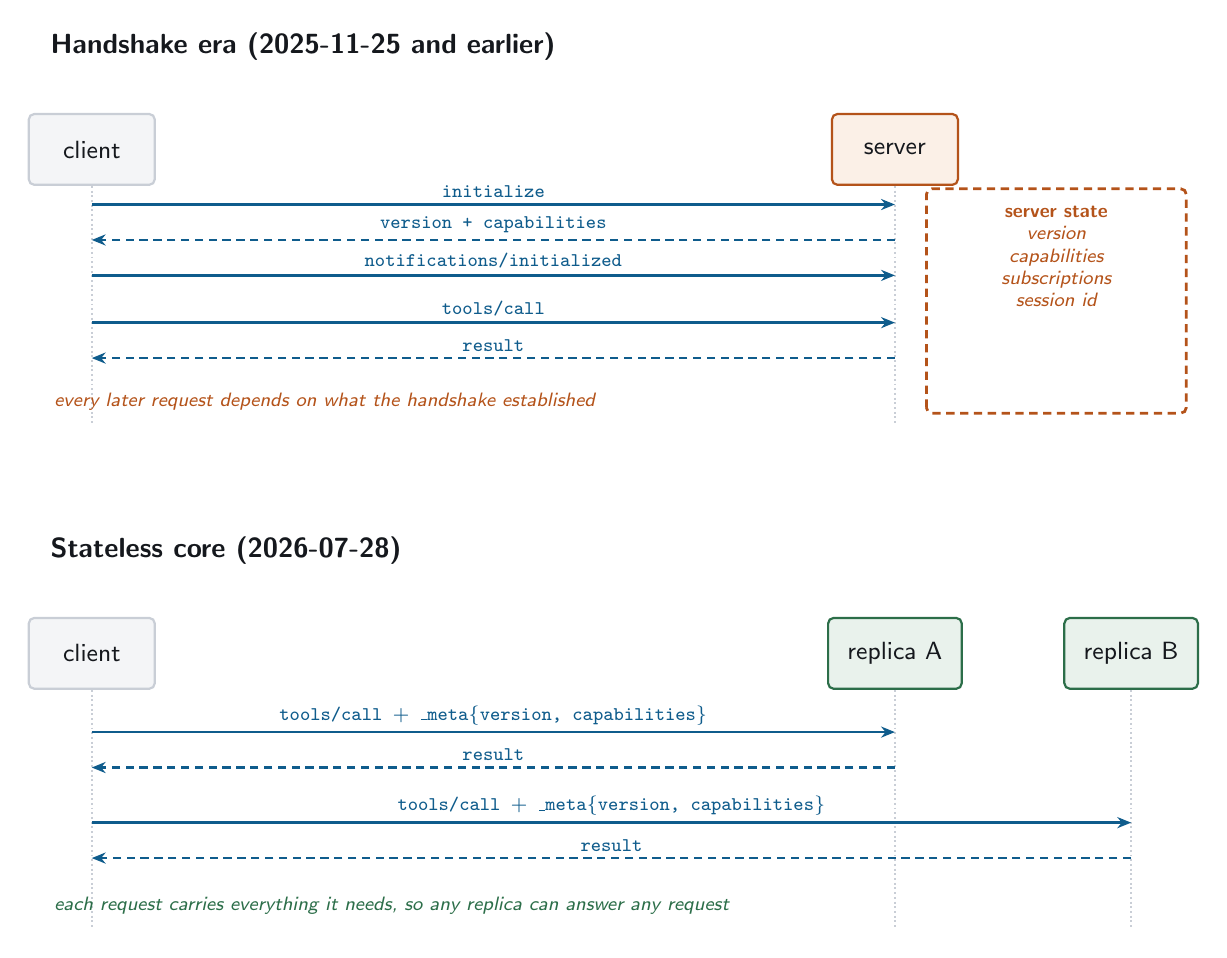
\begin{tikzpicture}[x=1cm, y=1cm]

% =========================================================================
% TOP: the 2025 handshake era
% =========================================================================
\begin{scope}[yshift=0cm]
  \node[lblink, font=\sffamily\bfseries, anchor=west] at (-0.6,3.5)
    {Handshake era (2025-11-25 and earlier)};

  \node[box, minimum width=16mm] (c) at (0,2.2) {client};
  \node[boxw, minimum width=16mm] (s) at (10.2,2.2) {server};
  \draw[lifeline] (c) -- (0,-1.3);
  \draw[lifeline] (s) -- (10.2,-1.3);

  \draw[flow] (0,1.5) -- node[tag, above] {initialize} (10.2,1.5);
  \draw[flow, densely dashed] (10.2,1.05)
        -- node[tag, above] {version + capabilities} (0,1.05);
  \draw[flow] (0,0.6) -- node[tag, above] {notifications/initialized} (10.2,0.6);

  % the session box
  \draw[draw=warm, line width=1pt, densely dashed, rounded corners=2pt]
    (10.6,-1.15) rectangle (13.9,1.7);
  \node[note, text=warm, align=center, anchor=north] at (12.25,1.6)
    {\textbf{server state}\\version\\capabilities\\subscriptions\\session id};

  \draw[flow] (0,0.0) -- node[tag, above] {tools/call} (10.2,0.0);
  \draw[flow, densely dashed] (10.2,-0.45) -- node[tag, above] {result} (0,-0.45);

  \node[note, text=warm, anchor=west] at (-0.6,-1.0)
    {every later request depends on what the handshake established};
\end{scope}

% =========================================================================
% BOTTOM: 2026-07-28
% =========================================================================
\begin{scope}[yshift=-6.4cm]
  \node[lblink, font=\sffamily\bfseries, anchor=west] at (-0.6,3.5)
    {Stateless core (2026-07-28)};

  \node[box, minimum width=16mm] (c2) at (0,2.2) {client};
  \node[boxg, minimum width=16mm] (s2a) at (10.2,2.2) {replica A};
  \node[boxg, minimum width=16mm] (s2b) at (13.2,2.2) {replica B};
  \draw[lifeline] (c2) -- (0,-1.3);
  \draw[lifeline] (s2a) -- (10.2,-1.3);
  \draw[lifeline] (s2b) -- (13.2,-1.3);

  \draw[flow] (0,1.2) -- node[tag, above, align=center]
    {tools/call \textnormal{+} \_meta\{version, capabilities\}} (10.2,1.2);
  \draw[flow, densely dashed] (10.2,0.75) -- node[tag, above] {result} (0,0.75);

  \draw[flow] (0,0.05) -- node[tag, above, align=center]
    {tools/call \textnormal{+} \_meta\{version, capabilities\}} (13.2,0.05);
  \draw[flow, densely dashed] (13.2,-0.4) -- node[tag, above] {result} (0,-0.4);

  \node[note, text=good, anchor=west, align=left] at (-0.6,-1.0)
    {each request carries everything it needs, so any replica can answer any request};
\end{scope}

\end{tikzpicture}
\end{document}
